%!  pour pdfLatex
\documentclass{beamer}

%\usepackage[pdftex]{graphicx,color}
%\usepackage[pdftex,colorlinks={true},urlcolor={blue},pdfauthor={remy Nicolai}]{hyperref}

\usepackage[utf8]{inputenc}
\usepackage[T1]{fontenc}
\usepackage{lmodern}
\usepackage[frenchb]{babel}

\usetheme{Warsaw}

%\usepackage{fancyhdr}
%\pagestyle{fancy}

%\usepackage{floatflt}
\usepackage{maths}

\usepackage{parcolumns}
\setlength{\parindent}{0pt}

%\usepackage{caption}
%\usepackage{subcaption}

\usepackage[french,ruled,vlined]{algorithm2e}
\SetKwComment{Comment}{\#}{}
\SetKwFor{Tq}{tant que}{}{}
\SetKwFor{Pour}{pour}{}{}
\DontPrintSemicolon
\SetAlgoLined

\usepackage{listings}
\lstset{language=Python,frame=single}

%pr{\'e}sentation des compteurs de section, ...
\makeatletter
\renewcommand{\thesection}{\Roman{section}.}
\renewcommand{\thesubsection}{\arabic{subsection}.}
\renewcommand{\thesubsubsection}{\arabic{subsubsection}.}
%\renewcommand{\labelenumii}{\theenumii.}
\makeatother


\newtheorem*{thm}{Théorème}
\newtheorem{thmn}{Théorème}
\newtheorem*{prop}{Proposition}
\newtheorem{propn}{Proposition}
\newtheorem*{pa}{Présentation axiomatique}
\newtheorem*{propdef}{Proposition - Définition}
\newtheorem*{lem}{Lemme}
\newtheorem{lemn}{Lemme}

\theoremstyle{definition}
\newtheorem*{defi}{Définition}
\newtheorem*{nota}{Notation}
\newtheorem*{exple}{Exemple}
\newtheorem*{exples}{Exemples}


\newenvironment{demo}{\renewcommand{\proofname}{Preuve}\begin{proof}}{\end{proof}}
%\renewcommand{\proofname}{Preuve} doit etre après le begin{document} pour fonctionner

\theoremstyle{remark}
\newtheorem*{rem}{Remarque}
\newtheorem*{rems}{Remarques}

%\usepackage{maths}
%\newcommand{\dbf}{\leftrightarrows}

%En tete et pied de page
%\lhead{Informatique}
%\chead{Introduction aux systèmes informatiques}
%\rhead{MPSI B Hoche}
%\lfoot{\tiny{Cette création est mise à disposition selon le Contrat\\ Paternité-Partage des Conditions Initiales à l'Identique 2.0 France\\ disponible en ligne http://creativecommons.org/licenses/by-sa/2.0/fr/
%} }
%\rfoot{\tiny{Rémy Nicolai \jobname}}

\nonstopmode

\begin{document}
\begin{frame}
\frametitle{Un algorithme en langage "naturel" (Ginette Mathiot)}
 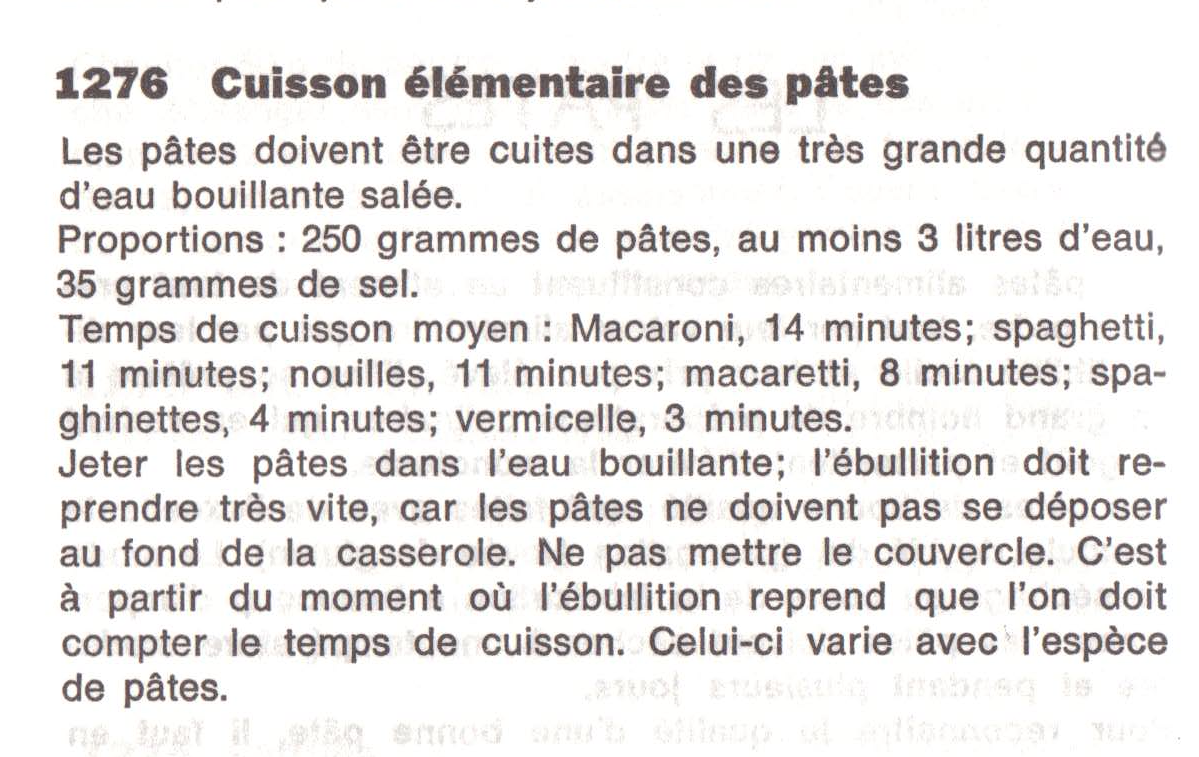
\includegraphics[width=9cm]{introalgo_1.png}  
\end{frame}

\begin{frame}[fragile]
  \frametitle{Présentation avec indentation}
\begin{verbatim}
utiliser : 250 g de pâtes, 35 g de sel, 3 litres d'eau
 -faire bouillir de l'eau salée
 -mettre les pâtes dans l'eau
 -laisser cuire 5mn
\end{verbatim} 
\end{frame}

\begin{frame}
  \frametitle{Concepts de base}
  \begin{description}
 \item[objet] modifiable (mutable) ou non. littéral (literals).
  \item[nom] un nom référence un objet, différent d'une variable, \emph{portée} (champ de validité)
 \item[expression] formée avec des littéraux, des noms, des opérateurs des parenthèses, peut être évaluée à un objet
 \item[référence] (assignation, "="),  à gauche nom,  à droite expression
 \item[fonction] une fonction "fait quelque chose" avec les paramètres qu'elle reçoit et \emph{renvoie} ou non un objet. Certaines fonctions sont des \emph{méthodes} d'un type d'objet.
\end{description}
\end{frame}

\begin{frame}
  \frametitle{Exemple de mise en \oe{}uvre}
  \begin{itemize}
    \item Cassy $\leftarrow$ une casserole\newline Eg $\leftarrow$ un égouttoir
    \item Cassy.ajouter(eau + sel)
    \item faireBouillir(Cassy)
    \item Cassy.ajouter(pâtes)
    \item chauffer(Cassy,5)
    \item Eg.ajouter(Cassy.vider())
    \item Eg.secouer()
    \item Cassy.ajouter(Eg.vider() + beurre)
    \item Eg.oublier()
  \end{itemize}
\end{frame}

\begin{frame}[fragile]
  \frametitle{Structures de contrôle}
\begin{itemize}
  \item \emph{branchement} \texttt{if} \index{structure de contrôle! branchement \texttt{if}}
  \item \emph{boucle} \texttt{while} \index{structure de contrôle! boucle \texttt{while}}
\end{itemize}
\begin{verbatim}
faireBouillir est une fonction de paramètre r
   si non bonAchauffer(r):
       terminer en renvoyant un message d'erreur
   tant que tempInt(r)< 100
       chauffer(r,1)
\end{verbatim}
\end{frame}

\begin{frame}[fragile]
  \frametitle{Syntaxe Python : \texttt{if}}
  Afficher "\texttt{ est entier}" si le nom \texttt{nono} désigne un entier et "\texttt{ est pas entier}" sinon.
\begin{verbatim}
#nono = "tagada"
#nono = 1
#nono  = "1"

if type(nono) == int:
    print "est entier"
else:
    print "est pas entier"
\end{verbatim}
\end{frame}

\begin{frame}[fragile]
  \frametitle{Syntaxe Python : \texttt{while}}
  Soit $b=16$ et $x=14578$, chercher le plus petit entier $n$ tel que $x < b^n$.
\begin{verbatim}
b = 16 
x = 14578
p = 1
n = 0

while p <= x:
    n = n + 1
    p = p * b
    
print(n)
print(x)
print(p)
\end{verbatim}
\end{frame}

\begin{frame}[fragile]
  \frametitle{Algorithme de numération : les grands d'abord}
  \begin{verbatim}
b = 10 ; x = 16**8 ; print(x)
#chercher plus gd b**n tq  b**n <= x (en deux temps)
p = 1 ; n = 0
while p <= x:
    n = n + 1
    p = p * b
p = p // b
#formation du développement
resultat = []
while x > 0 :
    resultat.append(x // p)
    x = x % p
    p = p // b
print(resultat)  
\end{verbatim}
\end{frame}

\begin{frame}[fragile]
  \frametitle{Algorithme de numération : les petits d'abord}
  \begin{verbatim}
b = 10 ; x = 16**8 ; print(x)
resultat = []
while x > 0 :
    resultat.append(x % b)
    x = x // b
print(resultat)  
\end{verbatim}
où est le problème?
\end{frame}

\begin{frame}
  \frametitle{Méthodes de liste}
  Pourquoi \newline
  \texttt{resultat.append()}\newline
  et pas\newline
  \texttt{resultat.prepend()} ?
  \newline (ou quelque chose de ce genre)
\end{frame}

\begin{frame}
  \frametitle{Définition de la partie entière}
D'après une propriété de $\R$, tout nombre réel se décompose de manière unique sous la forme
\begin{displaymath}
  \text{un nombre réel} = \text{un nombre entier} + \text{un nombre réel dans $[0,1[$}
\end{displaymath}
Notation
\begin{displaymath}
  x = \underset{\text{partie entière de } x\in \Z }{\underbrace{\lfloor x \rfloor}} + \underset{\in [0,1[ }{\underbrace{\{ x \}}}
\end{displaymath}
On dit aussi que $\{x\}$ est la partie \emph{décimale} de $x$.
\end{frame}

\begin{frame}
\frametitle{partie entière et division euclidienne}
$\Q$ est une partie de $\R$.

Division de $m\in \Z$ par $n\in \N^*$ 
\begin{displaymath}
  m = \underset{\in \Z}{\underbrace{n}}q + \underset{\in \llbracket 0, n\llbracket}{\underbrace{r}}
  \Leftrightarrow \frac{m}{n} = \underset{\in \N}{\underbrace{q}} + \underset{\in [0,1[}{\underbrace{\frac{r}{n}}} 
\end{displaymath}
Le quotient de la division de $m$ par $n$ est $\lfloor \frac{m}{n} \rfloor$.
\end{frame}

\begin{frame}
\frametitle{Développement d'un réel $x>0$}
\begin{algorithm}[H]
  $y\longleftarrow \lfloor x \rfloor$\;
  \Tq{ $y > 0$}{
      enregistrer le reste de la division de $y$ par $b$\;
      $y\longleftarrow $ le quotient de la division de $y$ par $b$\;
  }
  \caption{\`A gauche: les petits d'abord.}
  \label{nbbin_1}
\end{algorithm}
\bigskip
\begin{algorithm}[H]
  $y\longleftarrow \{ x \}$\;
  \Tq{ $y > 0$}{
      enregistrer $\lfloor by \rfloor$\;
      $y\longleftarrow \{ by\}$\;
  }
  \caption{\`A droite: les grands d'abord.}
  \label{nbbin_2}
\end{algorithm}
\end{frame}

\begin{frame}
  \frametitle{Exemple: $7.3$ en base $2$.}
  \begin{align*}
  \only<4->1 & & \only<3->1 & &\only<2->{1} & &. & & 
  \only<6->0 & & \only<7->1 & &\only<8->0 & & \only<9->0 & &
  \only<10->1 & &
  \end{align*}
  \only<1>{à gauche, les petits d'abord: $y\rightarrow 7$}
  \only<2>{$y\rightarrow 3$}
  \only<3>{$y\rightarrow 1$}
  \only<4>{$y\rightarrow 0$}
  \only<5>{à droite, les grands d'abord: $y\rightarrow 0.3$}
  \only<6>{$y\rightarrow 0.6$} \only<7>{$y\rightarrow 0.2$}
  \only<8>{$y\rightarrow 0.4$} \only<9>{$y\rightarrow 0.8$}
  \only<10>{$y\rightarrow 0.6$ et la séquence se répète $\cdots$} 
  \only<11>{$111.01001\,1001\,1001\,\cdots$}
\end{frame}

\begin{frame}
\frametitle{Questions mathématiques}
Le développement pratique montre qu'il existe des nombres 
\begin{displaymath}
a_1, a_2, \cdots, a_n \in \llbracket 0, b\llbracket, \hspace{0.5cm} y_n \in [0,1[  
\end{displaymath}
tels que 
\begin{displaymath}
  x = \lfloor x \rfloor + a_1b^{-1} + a_2b^{-2} + \cdots + + a_nb^{-n} + y_nb^{-n}  
\end{displaymath}

\begin{itemize}
  \item Dans quel cas l'algorithme de la partie droite se termine-t-il?
  \item Dans le cas où il ne se termine pas, la suite 
\begin{displaymath}
  \left( a_1b^{-1} + a_2b^{-2} + \cdots + + a_nb^{-n}\right)_{n\in \N^*}
\end{displaymath}
converge-t-elle ? vers $\{x\}$?
\end{itemize}  
\end{frame}

\begin{frame}
  \frametitle{Condition de terminaison}
Pour un $x$ donné, l'algorithme se termine si et seulement si il existe un entier $n$ tel que $xb^n \in \Z$.
\begin{align*}
  &\text{nombres binaires}:& &x\in \B \Leftrightarrow \exists n \in\N \text{ tel que } x\,2^{n} \in \Z \\
  &\text{nombres décimaux}:& &x\in \D \Leftrightarrow \exists n \in\N \text{ tel que } x\,10^{n} \in \Z 
\end{align*}
Un nombre décimal est-il binaire?\newline Un nombre binaire est-il décimal?
\end{frame}

\begin{frame}
  \frametitle{Développement en base $b$}

Si un $y_n = 0$, on choisit de poser $a_{n+1} = a_{n+2} = \cdots = 0$ de manière à former une suite de $a_k$ dans tous les cas.\newline

Pour chaque nombre réel dans $[0,1[$
\begin{itemize}
  \item L'algorithme associe une unique suite $\left( a_n\right)_{n\in \N}$ d'éléments de $\llbracket 0, b\llbracket$ appelé développement en base $b$.
  \item La suite  $\left( \left( a_1b^{-1} + a_2b^{-2} + \cdots + a_nb^{-n}\right)\right)_{n\in \N^*}$ converge vers le nombre donné.
  \item Deux nombres distincts ont des développements distincts
\end{itemize}
\end{frame}

\begin{frame}
  \frametitle{Attention aux nombres binaires ou décimaux}
\begin{displaymath}
  \left( \sum_{k=0}^n b^{-k} \right)_{n\in \N} \rightarrow \frac{1}{1-\frac{1}{b}} = \frac{b}{b-1}
  \Rightarrow 
  \left( \sum_{k=0}^n (b-1)b^{-k} \right)_{n\in \N} \rightarrow  b
\end{displaymath}
donc $x = a_1b^{-1} + \cdots + a_pb^{-p}$ avec $a_p>0$ est limite de la suite
\begin{multline*}
    a_1b^{-1} + \cdots +a_{p-1}b^{-p+1} + (a_p-1)b^{-p} \\
    + (b-1)b^{-p-1}+ (b-1)b^{-p-2} + \cdots + (b-1)b^{-n}
\end{multline*}
En base 10, le développement d'un décimal est stationnaire de valeur $0$. Il pourrait aussi s'écrire avec une infinité de $9$ par exemple 
\begin{displaymath}
 1.1199999999999999999999999\cdots = 1.1200000000\cdots = 1.12
\end{displaymath}
mais on évite de le faire.
\end{frame}

\begin{frame}
  \frametitle{Caractérisation des rationnels}
\begin{prop}
  Un nombre réel est rationnel (c'est à dire dans $\Q$) si et seulement si son développement en base $b$ est périodique à partir d'un certain rang.
\end{prop}
\end{frame}

\end{document}

